%% Beamer Template of Sabine Hauert and R.~Eddie Wilson
%% Available on https://www.overleaf.com/latex/templates/eddies-minimum-beamer-style/qhcyjdqkbbgx#.V-vfg1SLS1I
%%%%%%%%%%%%%%%%%%%%%%%%%%%%%%%%%%%%%%%%%%%%%%
% Head matter - can we try to be consistent on
% included packages
\documentclass{beamer}

\mode<presentation>
{\usetheme{default}
 \usecolortheme{default}
\usefonttheme{default}
\setbeamertemplate{navigation symbols}{}
\setbeamertemplate{caption}[numbered]} 
% Block colors
\setbeamercolor{block body}{bg=blue!10,fg=black}
\setbeamercolor{block title}{bg=blue!30,fg=black}
% Pour que tikzcd fonctionne
%\[\begin{tikzcd}[ampersand replacement=\&, column sep=small]\end{tikzcd}\]
\usepackage[frenchb]{babel}
\usepackage{amsfonts}
\usepackage{amsmath}
\usepackage{amssymb}
%\usepackage[T1]{fontenc}
\usepackage[utf8]{inputenc}
\usepackage{amsthm}
\usepackage{graphicx}
\usepackage{tikz}
\usepackage{tikz-cd}
\usepackage{hyperref}
\usepackage{amssymb}
\usepackage{geometry}

\hypersetup{                    % parametrage des hyperliens
    colorlinks=true,                % colorise les liens
    breaklinks=true,                % permet les retours à la ligne pour les liens trop longs
    urlcolor= blue,                 % couleur des hyperliens
    linkcolor= blue,                % couleur des liens internes aux documents (index, figures, tableaux, equations,...)
    citecolor= cyan               % couleur des liens vers les references bibliographiques
    }

\theoremstyle{definition}
\newtheorem{definition}{Definition}
\newtheorem{thm}{Theorem}
\newtheorem{ex}{Exercice}
\newtheorem{lem}{Lemma}
\newtheorem*{dem}{Proof}
\newtheorem{prop}{Proposition}
\newtheorem{cor}{Corollary}
\newtheorem{conj}{Conjecture}
\newtheorem{Res}{Result}
\newtheorem{Expl}{Example}
\newtheorem{rk}{Remark}

\newcommand{\N}{\mathbb N}
\newcommand{\Z}{\mathbb Z}
\newcommand{\R}{\mathbb R}
\newcommand{\C}{\mathbb C}
\newcommand{\Hil}{\mathcal H}
\newcommand{\Mn}{\mathcal M _n (\mathbb C)}
\newcommand{\K}{\mathbb K}
\newcommand{\B}{\mathbb B}
\newcommand{\Cat}{\mathbb B / \mathbb K}
\newcommand{\G}{\mathcal G }

\setlength\parindent{0pt}


%%%%%%%%%%%%%%%%%%%%%%%%%%%%%%%%%%%%%%%%%%%%%%
% Formatting for title page
\title[First Steps with SCRATCH]{Audition\\ \& AGPR}
\author{Clément Dell'Aiera}
\institute{University of Hawaii at Manoa}
\date{}
%%%%%%%%%%%%%%%%%%%%%%%%%%%%%%%%%%%%%%%%%%%%%%
\begin{document}

\begin{frame}
\titlepage
\begin{center} 
\includegraphics[width=3cm]{UH_logo.png}\end{center}
\end{frame}

\begin{frame}
  \tableofcontents\end{frame}

\section{Recherche}
\begin{frame}{Espaces m\'etriques}
\begin{definition}
Un espace m\'etrique d\'enombrable discret  $X$ est \`a \textit{g\'eom\'etrie born\'ee} si
\[\sup_{x\in X} | B(x,r)| < \infty \quad \forall r >0.\]
\end{definition}
\textit{Exemples typiques}\\
\vfill
\begin{itemize}
\item[$\bullet$] $X=(V,E)$ graphe de degr\'e uniform\'ement born\'e.
\vfill
\item[$\bullet$] $G=\langle S \rangle$ groupe finiment engendr\'e, muni de la \textit{m\'etrique des mots}\\
\[l(g) = \inf\{k : g = s_1 s_2 ... s_k , \ s_i \in S\}, \quad d(g,h) = l(g^{-1}h).\]
\end{itemize}
\vfill
($e_G\notin S$ et $S=S^{-1}$)
\end{frame}

\begin{frame}{Graphe de Cayley}
La m\'etrique des mots peut \^{e}tre r\'ealis\'ee comme une distance de graphe.\\
\vfill
\begin{definition}
Le \textit{Graphe de Cayley} associ\'ee au couple $(G,S)$ est 
\[|G| = (V,E_S)\]
avec : 
\vfill
\begin{itemize}
\item[$\bullet$] $V=G$,
\vfill
\item[$\bullet$] $(x,y)\in E_S$ ssi $x^{-1}y\in S$.
\end{itemize}
\end{definition}
\vfill
\end{frame}

\begin{frame}{$G=\Z$}
\[S= \{\pm 1\}\]
\begin{tikzpicture}
\scriptsize
\newcount\N;
\N 4; 

\foreach \i in {-6,...,\N}
	{
	\draw (\i+1,0) node{$\bullet$};
	\draw (\i+1,0) node[below]{$\i$};
     \draw (\i,0) -- (\i+ 1,0);
	}
 	\draw (\N+1,0) -- (\N+2,0);
 
 \foreach \i in {-3,...,\N/2}
		{
		\draw (2*\i+1,-3) node{$\bullet$};
		\draw (2*\i,-4) node{$\bullet$};
     		\draw (2*\i,-4) -- (2*\i+2,-4);
	 	\draw (2*\i,-4) -- (2*\i+3,-3);
	  	\draw (2*\i+1,-3) -- (2*\i+4,-4);
	 	\draw (2*\i+1,-3) -- (2*\i+3,-3);
	 	}
	 	\draw (-5,-3) -- (-6,-3);
	 	\draw (-4,-4) -- (-6,-3.3);
	 	\draw (-5,-3) -- (-6,-3.3);
 		 
\draw (-5,-3) node[above]{-5};
\draw (-3,-3) node[above]{-3};
\draw (-1,-3) node[above]{-1};
\draw (1,-3) node[above]{1};
\draw (5,-3) node[above]{5};
\draw (3,-3) node[above]{3};

\draw (0,-4) node[below]{0};
\draw (2,-4) node[below]{2};
\draw (-2,-4) node[below]{-2};
\draw (4,-4) node[below]{4};
\draw (-4,-4) node[below]{-4};
\draw (-6,-4) node[below]{-6};
\end{tikzpicture}
\[S= \{\pm 2 , \pm 3\}\]
\end{frame}

%\begin{frame}{$G=\mathbb F_2$}
%\begin{picture}(8.5cm,8.5cm)(-4.2cm,-4.2cm)
%\linethickness{1.5pt}
%{\A}
%{\B}
%{\C}
%{\D}
%\end{picture}
%\end{frame}

%\begin{frame}{$G=\mathbb F_2$}
%\begin{center}
%\begin{tikzpicture}
%\draw (0,0) node{$\bullet$};
%\foreach \i in {1,...,4}
%{
%	\draw (90*\i:2) node{$\bullet$};
 %     \draw (0,0) -- (90*\i: 2);      
%}
%\foreach \i in {1,...,4}
%{\foreach \a in {-1,...,1}
%{
%	\draw (90*\i:2)+(90*\a+90*\i:1) node{$\bullet$};
      %\draw (0,0) -- (90*\i: 1);      
%}}
%\end{tikzpicture}
%\end{center}
%\end{frame}

\begin{frame}{$G=\mathbb F_2 = \langle a,b\rangle$}
\begin{center}
\vfill
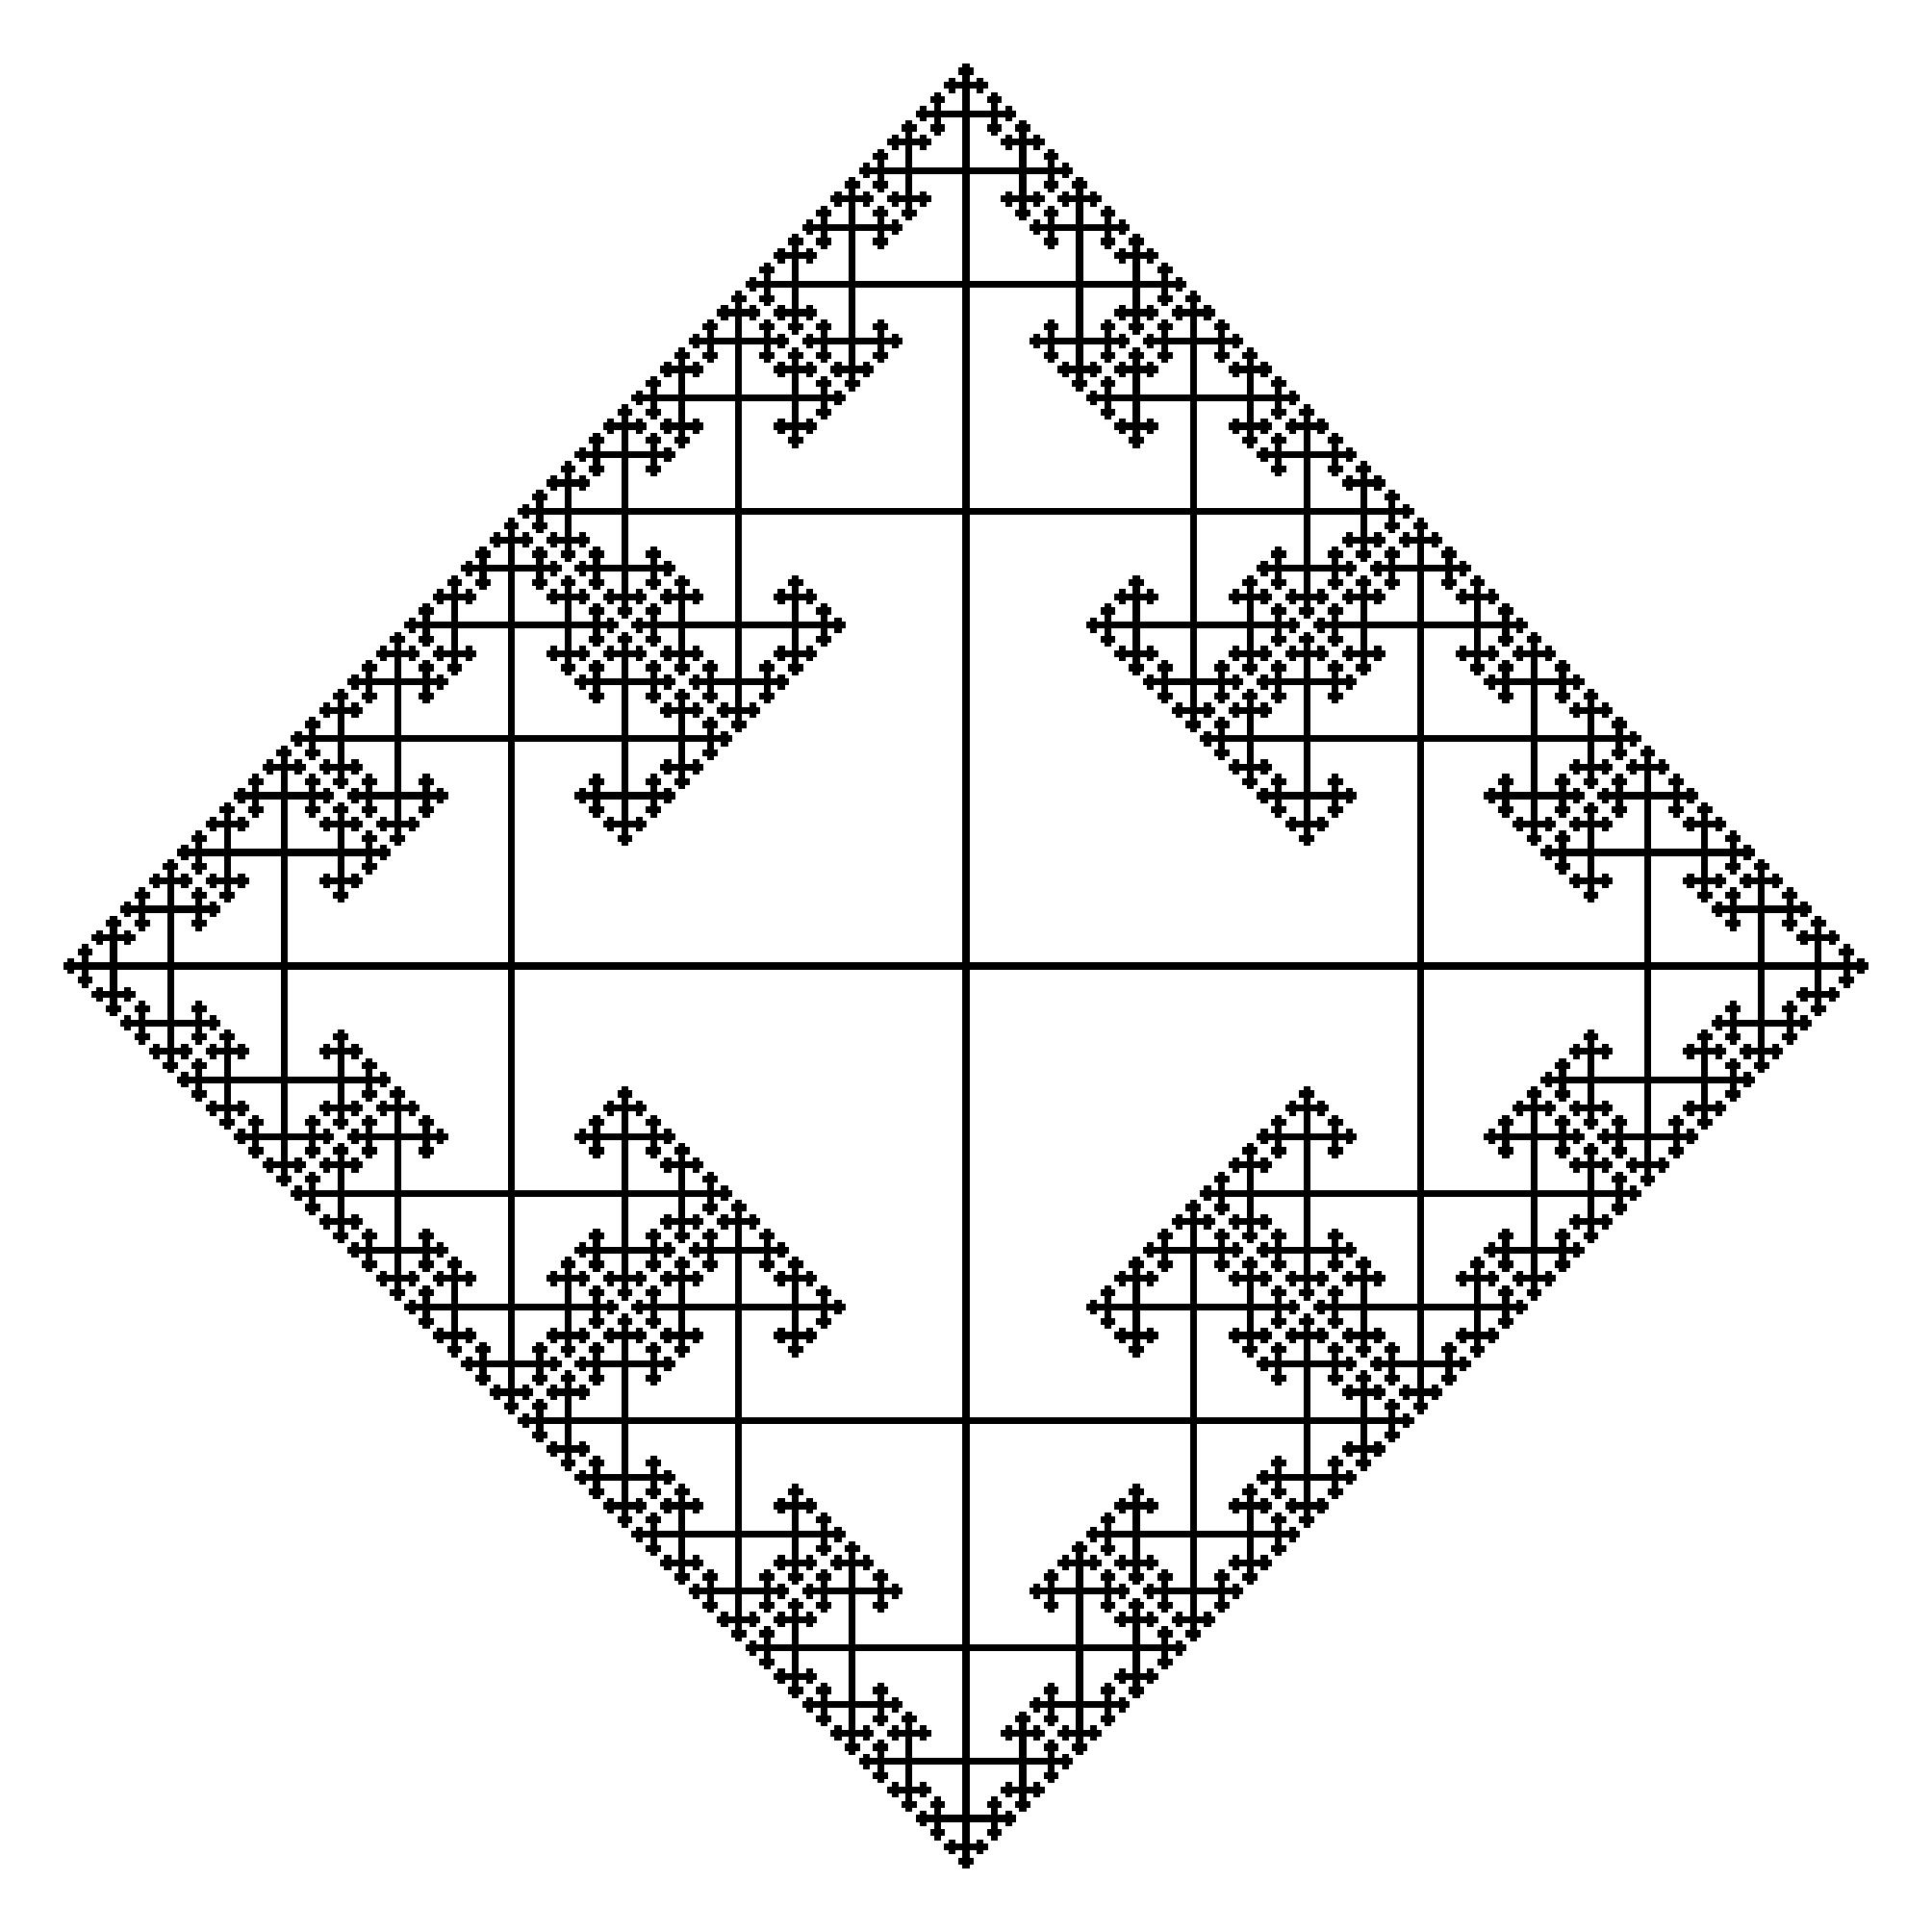
\includegraphics[width=0.8\linewidth]{Cayley_2}
\vfill
\end{center}
\end{frame}

%\begin{frame}
%\begin{center}
%\vfill
%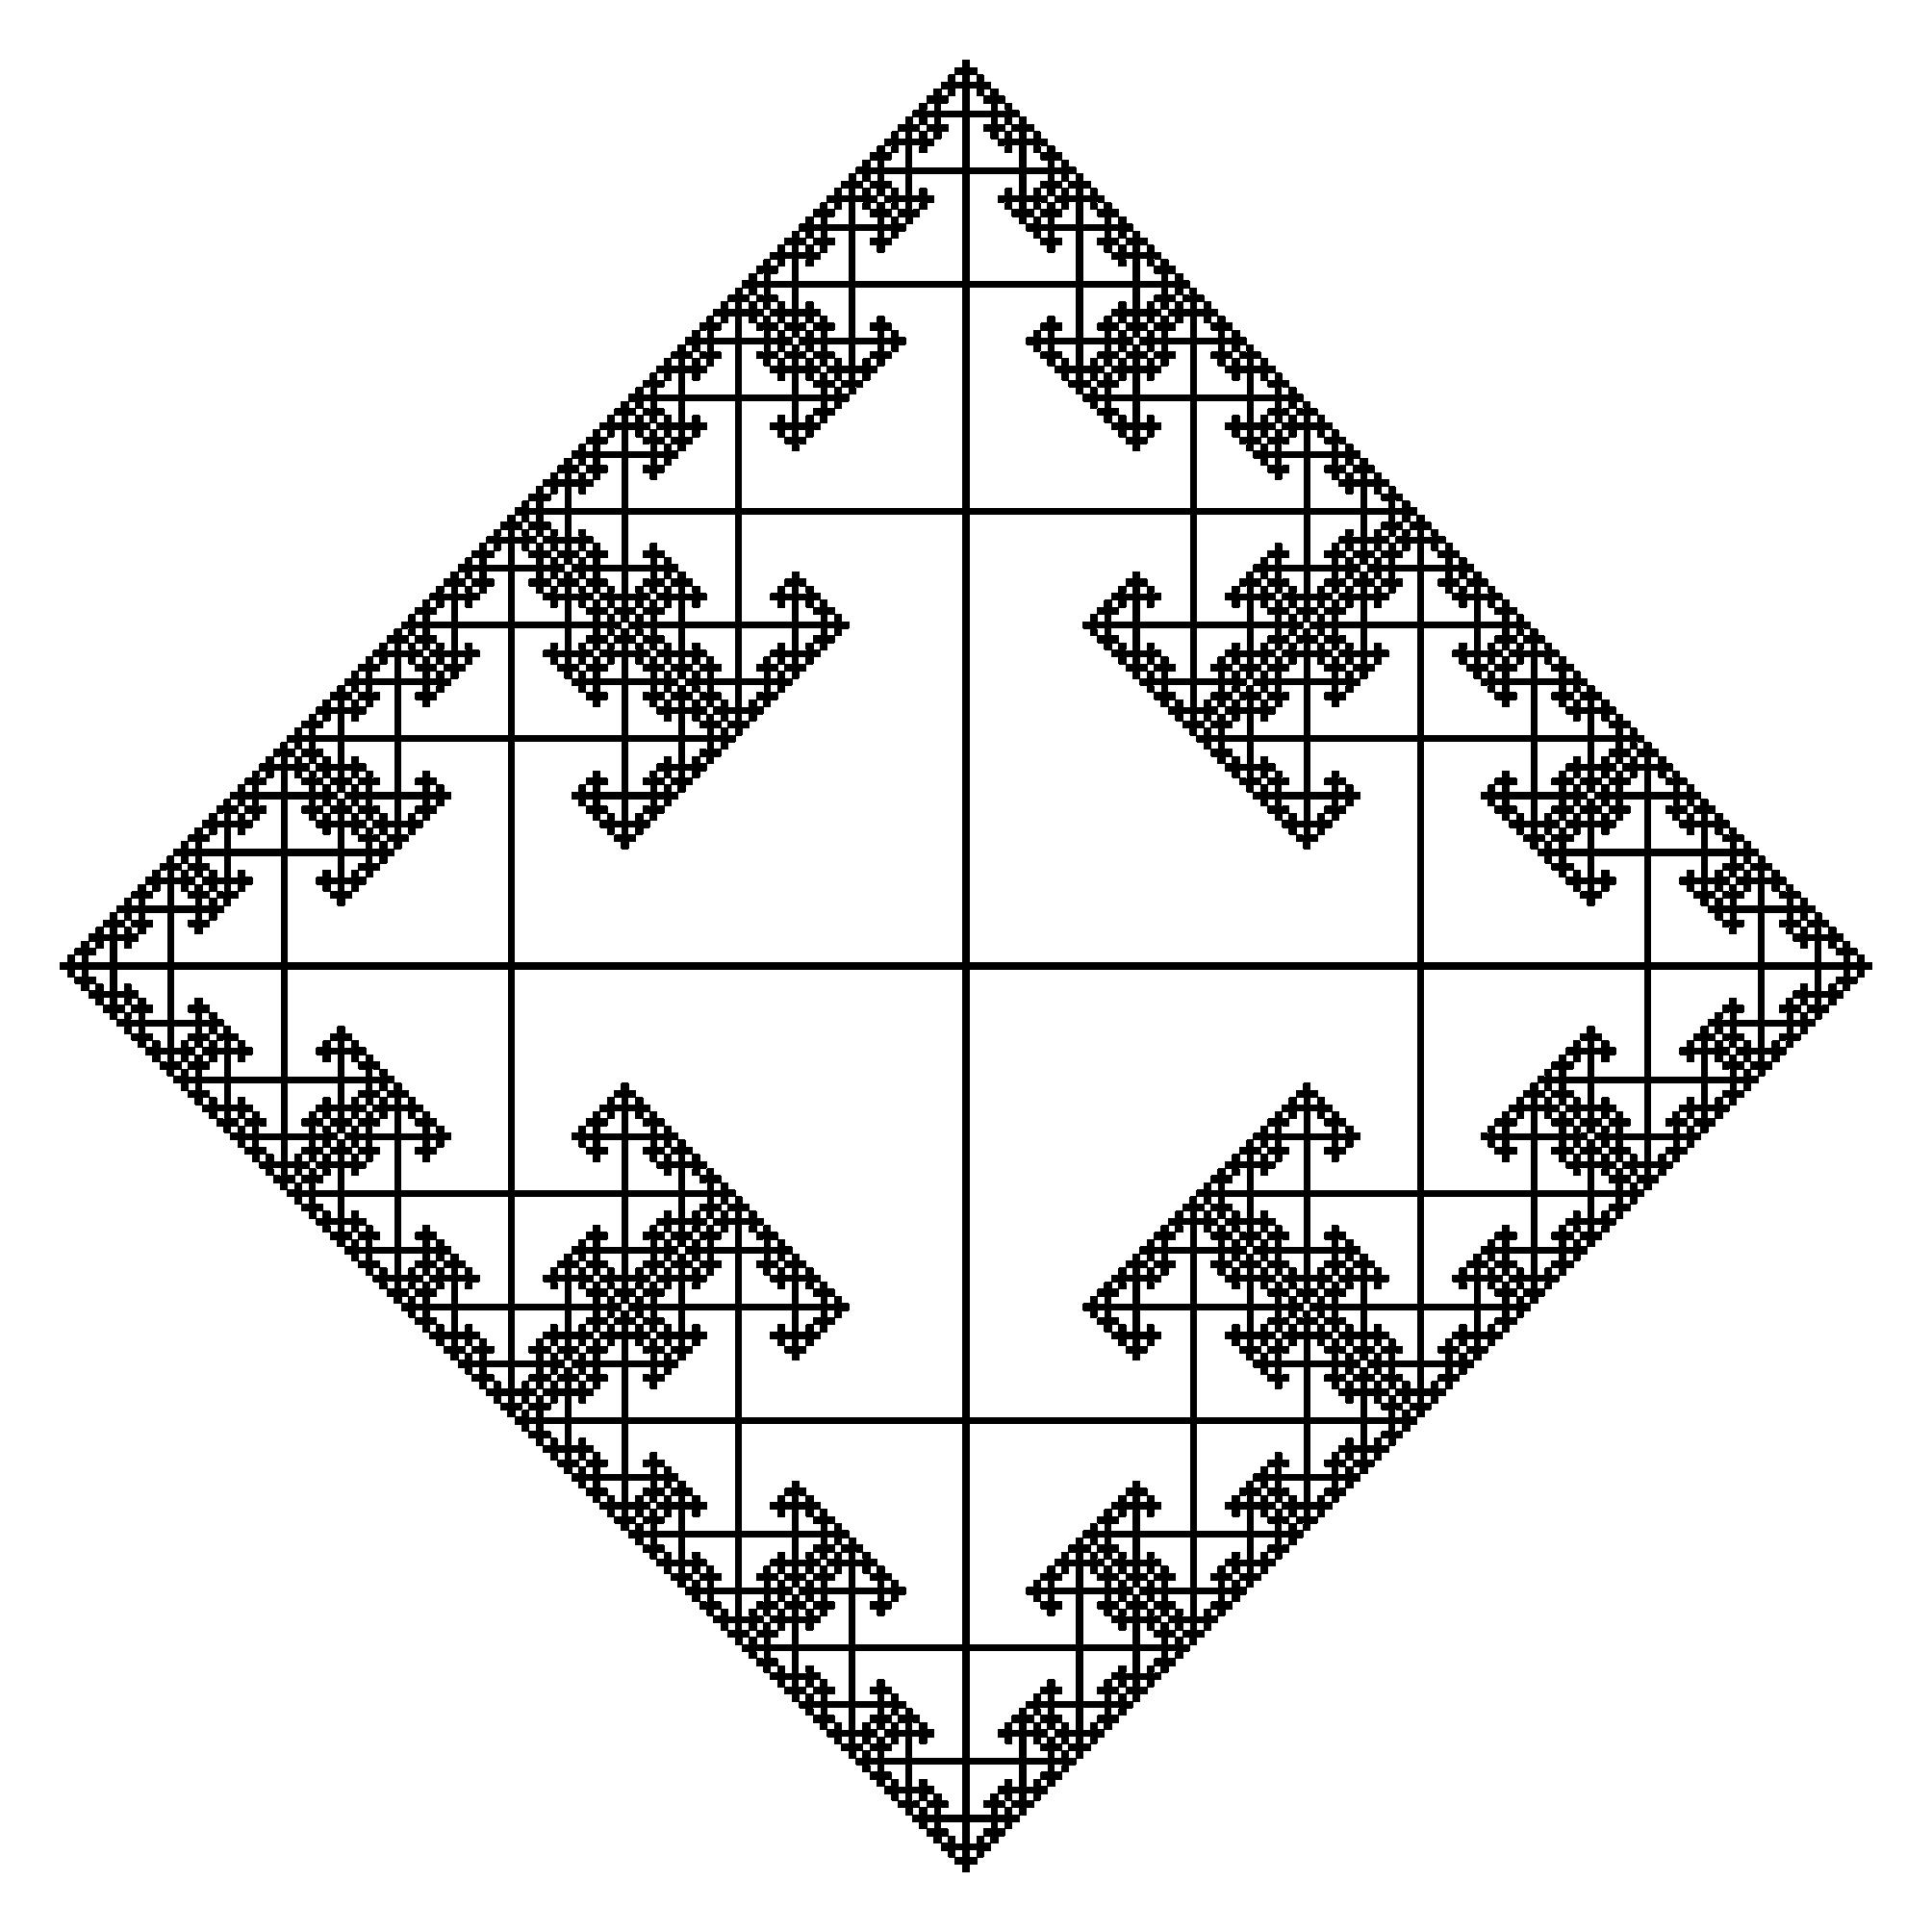
\includegraphics[width=0.8\linewidth]{Cayley}
%\vfill
%\end{center}
%\end{frame}

\begin{frame}{$G= \Z/(5)\ast \Z/(3) = \langle a,b \ : \ a^5, b^3\rangle$}
\begin{center}
\vfill
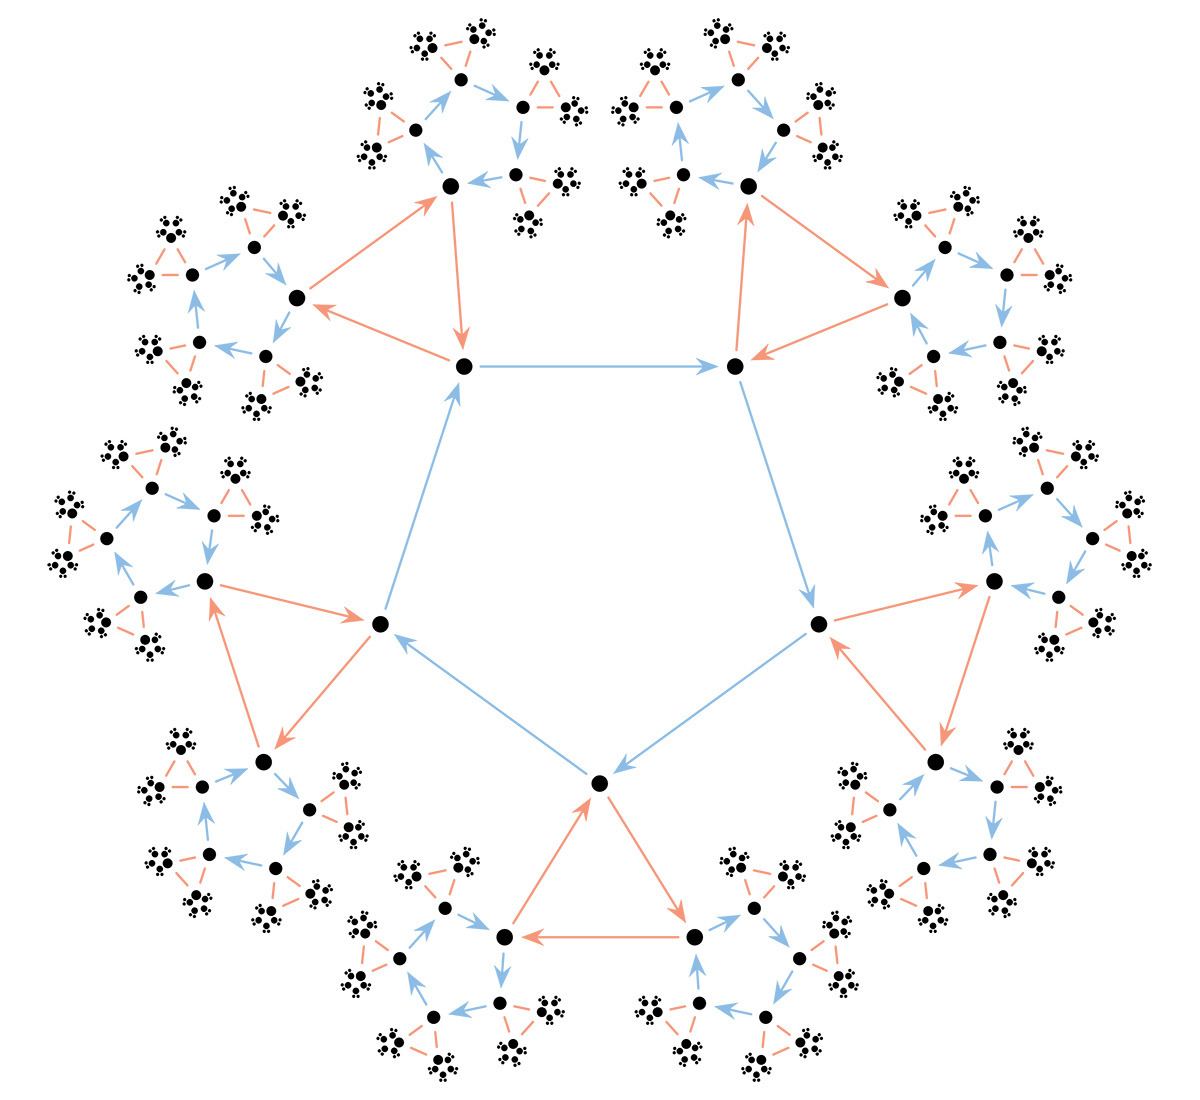
\includegraphics[width=0.8\linewidth]{PSL2}
\vfill
\end{center}
\end{frame}

%\begin{frame}{$G=PSL(2,\Z)$}
%\begin{center}
%\begin{tikzpicture}
%\scriptsize 
%\foreach \i in {1,...,3}
%{
%	\draw (120*\i:1) node{$\bullet$};
 %     \draw (120* \i : 1) -- (120*\i+120: 1);
%	\draw (120* \i : 1) -- (120*\i: 2);
      %}

%\foreach \j in {1,...,3}
%{\foreach \i in {1,...,3}
%{
%	\draw (120*\j:3)+(120*\i+60:1) node{$\bullet$};
%	\draw  (120*\j:3)+(120*\i+60:1) -- (120*\j:3)+(120*\i+180:1) -- (120*\j:3)+(120*\i+300:1) -- cycle;
      %\draw ((120*\j:3)+(120*\i+60:1)) -- ((120*\j:3)+(120*\i+180:1));
%}}
 %%\end{tikzpicture}
%\end{center}\end{frame}

\begin{frame}{Notations} 
\begin{block}{$l^2X=\overline{Vect_{\mathbb C} \{e_x\}_{x\in X}}$}
Il est muni du produit hermiten $\langle e_x, e_y\rangle =\delta_{xy}$. 
\end{block}
C'est un espace de Hilbert (complexe). La norme est \[\|x\| =\sqrt{\langle x, x\rangle}.\]
\begin{block}{$B(l^2X)$ d\'enote l'alg\`ebre des op\'erateurs lin\'eaires born\'es. }
La norme
\[\|a\| = \sup \{\ ||ax|| \ : \ \|x\| \leq 1 \} \] 
la munit d'une structure d'alg\`ebre de Banach.
\end{block}
\vfill
Pour $a\in B(l^2 X)$, on peut regarder les coefficients \[a_{xy} = \langle e_y, ae_x \rangle .\]
\end{frame}

\begin{frame}{Propagation finie}
On regarde \[\C_r [X] = \{ (a_{xy})\in B(l^2 X) \ : \ a_{xy }=0 \text{ si } d(x,y)> r\}  \]
Et 
\begin{block}{}
\[\C_u[X] = \cup_{r>0} \C_r[X] \subset B(l^2 X) \]
\end{block}
est la sous-alg\`ebre de $B(l^2 X)$ des op\'erateurs de \textit{propagation finie}.
\vfill
\textit{Exemple:} Si $X=(V,E)$ est un graphe, le Laplacien
\[(\Delta v)(x) = v(x) - \frac{1}{N_x}\sum_{x\sim y} v(y) \quad \forall v\in l^2(X)\]
est de propagation finie.
\end{frame}

\begin{frame}{Propagation finie}
\begin{center}
\vfill

\includegraphics[width=0.8\linewidth]{finite_propagation}
\vfill
%\captionof{figure}{\color{Green} A family of graphs}
\end{center}
\end{frame}

\begin{frame}{Alg\`ebre de Roe}
\begin{definition}
La compl\'etion de $\C_u[X]$ pour la norme d'op\'erateurs est appel\'ee \textit{l'alg\`ebre de Roe} de $X$. 
\end{definition}
\vfill
On la note $C^*_u(X)$.\\
\vfill
Int\'er\^{e}t: 
\begin{itemize}
\item[$\bullet$] th\'eor\`emes de l'indice \`a la Atiyah-Singer,
\item[$\bullet$] conjecture de Novikov,
\item[$\bullet$] conjecture de Baum-Connes.
\end{itemize}
\end{frame}

\begin{frame}{$K$-th\'eorie}
Donner un moyen de calculer les groupes de $K$-th\'eorie de $C^*_u(X)$.\\
\vfill
La $K$-th\'eorie d'une alg\`ebre de Banach $A$ est la donn\'ee de deux groupes ab\'eliens $K_0(A)$ et $K_1(A)$ qui sont des \'equivalents alg\'ebriques des groupes de cohomologie pour une vari\'et\'e par exemple.  
\vfill
R\^{o}le en classification.\\
\vfill

\end{frame}

\begin{frame}{$K$-th\'eorie}
Soit $H$ un espace de Hilbert s\'eparable.
\vfill
\begin{theorem}[2018 - Classification du programme d'Elliot ]
Les sous-alg\`ebres ferm\'ees $A$ de $B(H)$ qui sont
\begin{itemize}
\item[$\bullet$] approximables par des alg\`ebres de matrices (\textit{nucl\'eaires}),
\item[$\bullet$] simples,
\item[$\bullet$] r\'eguli\`eres (au sens d'une dimension finie),
\item[$\bullet$] satisfont le th\'eor\`eme dit UCT ,
\end{itemize}
sont classifi\'ees par des invariants provenant de la $K$-th\'eorie.
\end{theorem} 
\vfill
\textit{Le probl\`eme UCT}: \'Eliminer la derni\`ere hypoth\`ese.
\end{frame}

\begin{frame}{Probl\`eme UCT pour $C^*_u(\Z)$ (j.w.w. Amine Marrakchi)}
\begin{block}{Projet de recherche 1/2}
Prouver le th\'eor\`eme UCT pour $C^*_u(\Z)$.
\end{block}
\vfill
Pour cela, on plonge $C^*_u(X)$ dans son \textit{alg\`ebre \`a l'infini} $C^*_\infty(X)$.
\[ F_r = \prod_{n\in \mathbb N} \C_r[X] \subset l^\infty(\mathbb N , C^*_u(X))\]
\[C^*_\infty(X) = \overline{\cup_{r>0 } F_r} \ mod \ \bigoplus_n C^*_u(X)\]
\end{frame}

\begin{frame}{Probl\`eme UCT pour $C^*_u(\Z)$ (j.w.w. Amine Marrakchi)}
Pour $R$ tr\`es grand,
\begin{center}
\begin{tikzpicture}
\draw (4.5,1.5) node{$\Z$};
\draw[dashed] (0,1)--(10,1);
\foreach \i in {0,...,4}
	{
	\fill[blue!40!white](2*\i,0) rectangle (2*\i+1,0.3);
	\draw[blue] (2*\i,0) -- (2*\i+1,0);
	}
\foreach \i in {0,...,4}
	{
	\fill[red!40!white](2*\i+1,0) rectangle (2*\i+2,0.3);
	\draw[red] (2*\i+1,0) -- (2*\i+2,0);
	}
\draw[<->] (4,-0.5) -- (5,-0.5);
\draw (4.5,-0.5) node[below]{$10R$};
\end{tikzpicture}
\end{center}
\begin{itemize}
\item Choisir $r_n>0$ croissante telle que $\lim_n r_r = +\infty$.
\item $X_n$ partie bleue, et $Y_n$ partie rouge.
\end{itemize}
\[ B_r= \prod_n \C_r[X_n] \subset l^\infty (\mathbb N , C^*_u(\Z))\]
\[\mathcal B = \overline{\cup_{r>0} B_r}\]
De m\^eme pour $\{Y_n\}$ donne $R_r$ et $\mathcal R$.
\end{frame}

\begin{frame}{Probl\`eme UCT pour $C^*_u(\Z)$ (j.w.w. Amine Marrakchi)}
L'image de $C^*_u(\Z)$ dans $C^*_\infty(\Z)$ est \textit{d\'ecomposable} en deux id\'eaux bilat\`eres ferm\'es.
\vfill
\begin{block}{Mayer-Vietoris}
Un r\'esultat classique de topologie alg\'ebrique ram\`ene la preuve de UCT \`a celle de UCT pour $\mathcal B$ et $\mathcal R$.
\end{block}
\vfill
Cela d\'ecoule du fait que UCT soit vrai pour les matrices.
\end{frame}

\begin{frame}{Probl\`eme UCT pour $C^*_u(\Z)$ (j.w.w. Amine Marrakchi)}
\begin{block}{Projet de recherche 2/2}
Prouver le th\'eor\`eme UCT pour les $C^*$-alg\`ebres de dimension nucl\'eaire finie.
\end{block}
\vfill
Int\'er\^et: 
\vfill
\begin{itemize}
\item solution possible du probl\`eme UCT.
\vfill
\item classification des $C^*$-alg\`ebres de Roe.
\vfill
\item formalisation et conceptualisation de la $K$-th\'eorie quantitative.
\vfill
\end{itemize}
\end{frame}

\section{Agr\'egation}
\begin{frame}
  \tableofcontents[currentsection]
\end{frame}
\begin{frame}{Exp\'erience}

\begin{itemize}
\item[$\bullet$] Agr\'egation 2013, pr\'eparation de l'ENS Rennes
\vfill
\item[$\bullet$] Exp\'erience en enseignement pr\'epa Agr\'egation
\vfill
\begin{itemize}
\item[$\bullet$] Le\c{c}ons d'Analyse 
\vfill
\item[$\bullet$] TP de Mod\'elisation (option \textit{Statistiques}) 
\vfill
\end{itemize}
\item[$\bullet$] Autres cours pertinents
\vfill
\begin{itemize}
\item[$\bullet$] TP de Calcul Symbolique en Sage 
\vfill
\item[$\bullet$] TP et TD dans le Master de \textit{Math\'ematiques appliqu\'ees} de l'Universit\'e de Lorraine 
\vfill
\end{itemize}
\end{itemize}

\end{frame}

\begin{frame}{Cours sugg\'er\'es}
\begin{block}{Langages de programmation}
R, Python, Sage, Scilab.
\end{block}
\vfill
\begin{itemize}
\item compositions (AP ou MG),
\vfill
\item le\c{c}ons d'analyse et probabilit\'es,
\vfill
\item le\c{c}ons d'alg\`bre et g\'eom\'etrie,
\vfill
\item mod\'elisation option probabilit\'ees et statistiques
\end{itemize}
\vfill
\end{frame}

\footnotesize

%\begin{frame}{References}
%\bibliographystyle{plain}
%\bibliography{biblio}
%\end{frame} 

\Large
\begin{frame}{}
Merci de votre attention !
\end{frame}
\end{document}